\section{Traditional Notebooks}



We will now describe how a data scientist would perform this analysis with a traditional interactive notebook that uses Python. While we do so, we will describe the issues that arise.

\noindent {\bf Setting up and interacting  with third-party utility libraries - Security concerns.} Before even starting working on any of the afore-mentioned tasks the data analyst must make sure that all third-party python packages that will be used for retrieving and visualizing data, are installed. This step will either introduce a dependency between the analyst and some system administrator, or the analyst will need the appropriate access rights in order to perform the installation, typically, using a command line. The latter can be a security concern (especially, if the server on which the notebook operates, also hosts other applications) and can also lead to corrupted systems if not performed correctly. The complexity of this step increases as the number of utility libraries, our analyst wants to use, increases. \eat{More specifically, for cases when an analyst needs to access data stored in a MongoDB and a MySQL database, two drivers will need to be installed.}

\begin{figure*}[hbt!]
\centering
	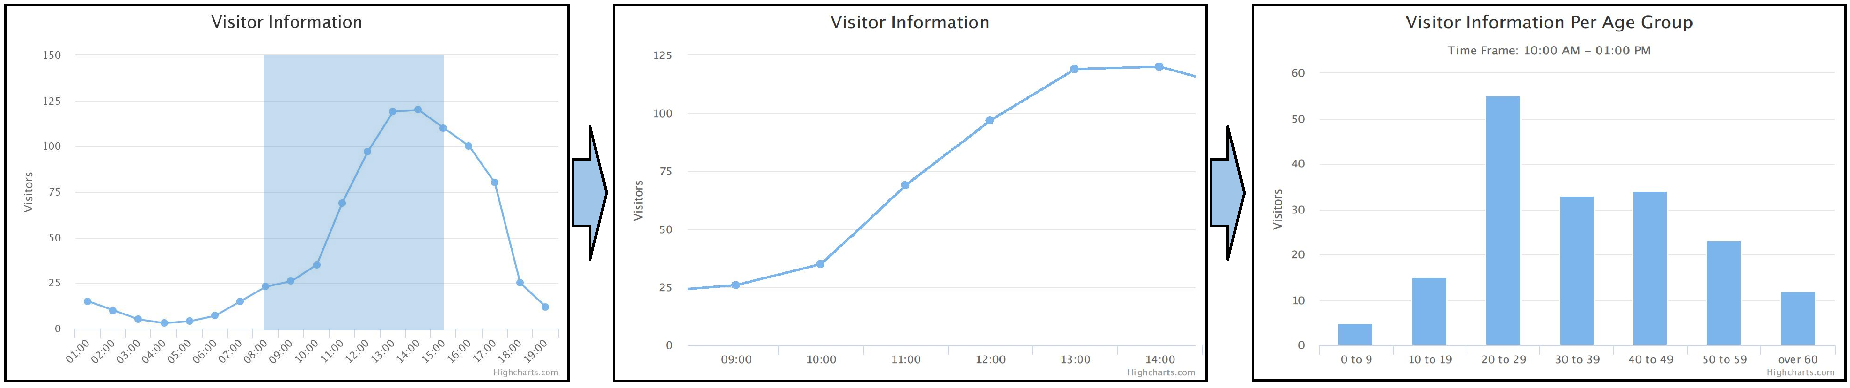
\includegraphics[width=1\textwidth]{figures/reactive-processing2.pdf}
	\caption{Demonstration of reactive charts. The reader's selection automatically updates both charts.}
	\label{fig:reactive-data-processing}
\end{figure*}


Once the system is configured, the analyst needs to read lengthy documentation pages in order to properly issue queries to the employed database system, using the API of the respective library. This step typically requires the use of imperative code that interacts with the library. During this step, the analyst has to also specify the credentials that will be used for accessing the database system. In most such libraries, the credentials have to be inlined into the method call that establishes the connection with that system. While this would not be a security concern in a python (or any other) application (since the code that includes the credentials would have been compiled into a binary file, thus hiding the credentials), in a python notebook, the credentials would lie in plain sight for anyone, who has access to the notebook, to see.

\noindent {\bf Data model conversions.}
After, establishing the connection with the database system, and issuing the queries, the analyst, is able to consume the results by using the internal, to the library, datamodel. After doing so, the analyst has to again read documentation pages in order to infer the data model dictated by the visualization library she selected, and manually perform the appropriate conversions in order to construct the first visualization, by invoking the appropriate renderer function. Note that data model conversions have to take place every time the analyst wishes to integrate a third-party library in her analysis, so the amount of plumbing code required, can quickly skyrocket.


\noindent {\bf Limited interactive exploratory capabilities.}
The next step, is for the analyst to issue a query that counts the visitors per age group for a set of selected hours and construct a bar chart showing the result. Note, however, that there's no straightforward way for selecting a meaningful time frame. The analyst will have to go through a process of trial and error, by issuing an arbitrary number of such queries and plotting the results, until she finds a set that produces valuable insight. Furthermore, even if the analyst goes through this process for the data corresponding to a particular day, the time frame selection she made, might not produce any valuable insight for the dataset corresponding to another day. Additionally, the reader cannot test further hypotheses that might come up.

\subsection*{Discussion about reactive charts} The use of co-dependent reactive charts would have been proven useful in this scenario. If the analyst was able to use a chart that allows the reader to select a particular range of hours by using the first plot, she could use that input in order to retrieve and plot only the user demographics for this particular range. Figure \ref{fig:reactive-data-processing} graphically depicts this process. The first figure shows the reader of the notebook, selecting a particular time frame; this causes the line chart to zoom in, thus showing only the selected time frame. After the reader performs the selection on the first chart, the subsequent bar chart is also updated thus only showing the age groups of the users that visited the portal during the selected time frame. This feature would add useful exploratory capabilities, to the notebook, which would be of great value to notebook readers. It would enable them to further analyze the underlying dataset used by the notebook by simply interacting with the provided visualizations. 

It is important to note that this feature cannot be implemented currently in interactive notebooks. Instead, the analyst would have to implement a full blown application in order to enable non-technical users interact with visualizations in this way. This requires more time and effort as well as technical expertise with web frameworks that data analysts, might lack. This reactive behavior requires the implementation of actions that have to be invoked when particular mouse events take place on the pixels of the browser that correspond to the visualization. Additionally, such events have to take place in a specific order (mousedown-mousemove-mouseup) for the action to be invoked. The developer of such applications must install observers that listen for such events and then provide the application logic that asynchronously accesses the back-end database to retrieve new data based on the user's selection and then cause the appropriate mutations to the respective visualizations that depend on that data. 


 % Template and template instance figures
 \begin{figure*}[hbt!]
 \centering
 %
 %
 \begin{minipage}[c]{6cm}
 %
 \begin{minipage}[c]{6.5cm}
 \begin{code}
 \textbf{<\% let} readings = 
    SELECT count(time) as visits, time
    FROM (SELECT * FROM page_views pv 
   	     join visitors v 
          on pv.v_id = v.vid) AS joined_table
    GROUP BY time 
    ORDER BY time ASC \textbf{\%>}
 \end{code}
 \vspace*{-0.4cm}
 \subcaption{Data retrieval}
 \label{figure:first-running-example:data-retrieval}
 \vspace*{0.3cm}
 \end{minipage}
 
 
 
 \begin{minipage}[c]{6.5cm}
 \begin{code}
 readings = [
    \{visits: 15, time: '08:00'\}, 
    \{visits: 10, time: '09:00'\},
    \{visits: 25, time: '10:00'\},  ...]
 \end{code}
 \vspace*{-0.4cm}
 \subcaption{Query Result}
 \label{figure:running-example:query-result}
 \vspace*{0.3cm}
 \end{minipage}
 
 
 \begin{minipage}[c]{6.5cm}
 \begin{code}
 sources : [ \{ 
      driver   : "postgres", 
      host     : "edu.db.domain", 
      expose   : [ \{
       schema : 'website_info', 
       tables: [visits, page_views] \} ]
      port     : 5432, 
      username : "dbadmin" 
      password : 'myP@ss'
    \}] 
 \end{code}
 \vspace*{-0.4cm}
 \subcaption{DB Access Configuration file}
 \vspace*{0.3cm}
 \label{figure:source-config-file}
 \end{minipage}
 %
 \vspace*{0.6cm}
 \end{minipage}
 \hspace{2cm}
 \begin{minipage}[c]{6cm}
 \begin{minipage}[c]{7.5cm}
 \begin{code}
   \directive{unit}{highcharts} \{
     title: 'Visitor information' ,
     type: 'line',
     xAxis : \{ 
       labels : ['08:00','09:00'...],
       min : '08:00'
       max : '22:00'
     \}
     series: [\{ data: [ \{y:15\}, \{y:10\}...] \}]
   \} \directive{end unit}{}
 \end{code}
 \vspace*{-0.4cm}
 \subcaption{Unit with evaluated unit state}
 \vspace*{0.3cm}
 \label{figure:running-example:unit-body}
 \end{minipage}
 \begin{minipage}[c]{7.5cm}
 \begin{code}
   \directive{unit}{highcharts} \{
     title: 'Visitor information',
     type: 'line',
     xAxis : \{ 
       labels : [
         \directive{for}{reading \textbf{in} readings} 
           \directive{print}{reading.time} 
         \directive{end for}{}],
       min : \directive{bind}{min_time},
       max : \directive{bind}{max_time}
     \}
     series: [\{
       data: [ \directive{for}{reading \textbf{in} readings}
           \{
             y  : \directive{print}{reading.count}
           \}
         \directive{end for}{} ]
     \}]
   \} \directive{end unit}{}
 \end{code}
 \vspace*{-0.3cm}
 \subcaption{Template \texttt{temp\_view}}
 \vspace*{0cm}
 \label{figure:first-running-example:main-template}
 \end{minipage}
 \end{minipage}
 \vspace*{-0.3cm}
 \caption{Template, template instance, and UAS configuration file for the running example}
 \vspace*{-0.3cm}
 \end{figure*}
